% The document class supplies options to control rendering of some standard
% features in the result.  The goal is for uniform style, so some attention 
% to detail is *vital* with all fields.  Each field (i.e., text inside the
% curly braces below, so the MEng text inside {MEng} for instance) should 
% take into account the following:
%
% - author name       should be formatted as "FirstName LastName"
%   (not "Initial LastName" for example),
% - supervisor name   should be formatted as "Title FirstName LastName"
%   (where Title is "Dr." or "Prof." for example),
% - degree programme  should be "BSc", "MEng", "MSci", "MSc" or "PhD",
% - dissertation title should be correctly capitalised (plus you can have
%   an optional sub-title if appropriate, or leave this field blank),
% - dissertation type should be formatted as one of the following:
%   * for the MEng degree programme either "enterprise" or "research" to
%     reflect the stream,
%   * for the MSc  degree programme "$X/Y/Z$" for a project deemed to be
%     X%, Y% and Z% of type I, II and III.
% - year              should be formatted as a 4-digit year of submission
%   (so 2014 rather than the accademic year, say 2013/14 say).

\documentclass[ % the name of the author
                    author={Dominic Joseph Moylett},
                % the degree programme
                    degree={MEng},
                % the dissertation    title (which cannot be blank)
                     title={Dictionary Matching with Fingerprints},
                % the dissertation subtitle (which can    be blank)
                  subtitle={An Empirical Analysis},
                % the dissertation     type
                      type={Research},
                % the year of submission
                      year={2014} ]{dissertation}

\begin{document}

% This macro creates the standard UoB title page by using information drawn
% from the document class (meaning it is vital you select the correct degree 
% title and so on).

\maketitle

% After the title page (which is a special case in that it is not numbered)
% comes the front matter or preliminaries; this macro signals the start of
% such content, meaning the pages are numbered with Roman numerals.

\frontmatter

% This macro creates the standard UoB declaration; on the printed hard-copy,
% this must be physically signed by the author in the space indicated.

\makedecl

% LaTeX automatically generates a table of contents, plus associated lists 
% of figures, tables and algorithms.  The former is a compulsory part of the
% dissertation, but if you do not require the latter they can be suppressed
% by simply commenting out the associated macro.

\tableofcontents
\listoffigures
\listoftables
\listofalgorithms
\lstlistoflistings

% The following sections are part of the front matter, but are not generated
% automatically by LaTeX; the use of \chapter* means they are not numbered.

% -----------------------------------------------------------------------------

\chapter*{Executive Summary}

{\bf A compulsory section, of at most $1$ page} 
\vspace{1cm} 

\noindent
This section should pr\'{e}cis the project context, aims and objectives,
and main contributions and achievements; the same section may be called
an abstract elsewhere.  The goal is to ensure the reader is clear about 
what the topic is, what you have done within this topic, {\em and} what 
your view of the outcome is.

The former aspects should be guided by your specification: essentially 
this section is a (very) short version of what is typically the first 
chapter.  The latter aspects should be presented as a concise, factual 
bullet point list.  The points will of course differ for each project, 
but an example is as follows:

\begin{quote}
\noindent
\begin{itemize}
\item I spent $120$ hours collecting material on and learning about the 
      Java garbage-collection sub-system. 
\item I wrote a total of $5000$ lines of source code, comprising a Linux 
      device driver for a robot (in C) and a GUI (in Java) that is 
      used to control it.
\item I designed a new algorithm for computing the non-linear mapping 
      from A-space to B-space using a genetic algorithm, see page $17$.
\item I implemented a version of the algorithm proposed by Jones and 
      Smith in [6], see page $12$, corrected a mistake in it, and 
      compared the results with several alternatives.
\end{itemize}
\end{quote}

\chapter*{Supporting Technologies}

\begin{quote}
\begin{itemize}
\item I used the GNU Multiple Precision Arithmetic Library (GMP) to support my implementation of Karp-Rabin fingerprints.\url{https://gmplib.org/}
\item I used the C Minimum Perfect Hashing Library (CMPH) for static perfect hashing.\url{http://cmph.sourceforge.net/}
\item I used an open-source implementation of Red-Black Trees from \url{http://en.literateprograms.org/Red-black_tree_(C)?oldid=19567}, with some minor adaptations.
\item The algorithms were tested against 50MB of gene DNA sequences from the Pizza and Chili Corpus.\url{http://pizzachili.dcc.uchile.cl/texts/dna/}
\end{itemize}
\end{quote}

% -----------------------------------------------------------------------------

\chapter*{Notation and Acronyms}

\begin{quote}
\begin{tabular}{lcl}
CMPH &: & C Minimum Perfect Hashing Library \\
GMP &: & GNU Multiple Precision Arithmetic Library \\
VO &: & A Viable Occurrence, a portion of the text which might match a pattern \\
KMP &: & The Knuth-Morris-Pratt single pattern matching algorithm \\
BST &: & Binary Search Tree \\
RBT &: & Red-Black Tree, a specific instance of a binary search tree \\
CLRS &: & Introduction to Algorithms by Thomas H. Cormen, Charles E. Lieserson, Ronald L. Rivest and Clifford Stein \\
$T$ &: & A text string of $n$ characters \\
$t_i$ &: & The $i$-th character in T \\
$\mathcal{P}$ &: & A list of $k$ patterns \\
$P_i$ &: & The $i$-th pattern in $\mathcal{P}$, a text string of $m_i$ characters \\
$M$ &: & A list of the length of each pattern in $\mathcal{P}$. \\
$p_{i,j}$ &: & The $j$-th character in $P_i$ \\
$|S|$ &: & The length of a string $S$ \\
$\phi(S)$ &: & The Karp-Rabin fingerprint of a string $S$ \\
$\rho_S$ &: & The period of a string $S$ \\
\end{tabular}
\end{quote}

% -----------------------------------------------------------------------------

\chapter*{Acknowledgements}

First and foremost, I would like to thank my supervisors: Dr. Rapha\"{e}l Clifford and Dr. Benjamin Sach. This project would have been impossible without their work and advice. Alongside them, I would like to mention Dr. Markus Jalsenius for his assistance during the summer project that led to this work and Dr. Allyx Fontaine, who contributed to the paper on which my project is based and advised me alongside Benjamin every week.

Everyone on my course has had an impact on me over the past four years. In particular, I would like to mention William Coaluca, Stephen de Mora, Nicholas Phillips, James Savage and Ashley Whetter. I have put countless hours into many projects with one or more of them.

I would like to acknowledge David Beddows, Derek Bekoe, Timothy Lewis and Jonathan Walsh for remaining a stable household for the past three years--four in the case of David and Timothy.

Last, but most certainly not least, I would like to thank my family and friends for the infinite support, happiness and love they have given me my entire life.

% =============================================================================

% After the front matter comes a number of chapters; under each chapter,
% sections, subsections and even subsubsections are permissible.  The
% pages in this part are numbered with Arabic numerals.  Note that:
%
% - A reference point can be marked using \label{XXX}, and then later
%   referred to via \ref{XXX}; for example Chapter\ref{chap:context}.
% - The chapters are presented here in one file; this can become hard
%   to manage.  An alternative is to save the content in seprate files
%   the use \input{XXX} to import it, which acts like the #include
%   directive in C.

\mainmatter

% -----------------------------------------------------------------------------

\chapter{Contextual Background}
\label{chap:context}

{\bf A compulsory chapter, of roughly $10$ pages}
\vspace{1cm} 

\noindent
This chapter should describe the project context, and motivate each of
the proposed aims and objectives.  Ideally, it is written at a fairly 
high-level, and easily understood by a reader who is technically 
competent but not an expert in the topic itself.

In short, the goal is to answer three questions for the reader.  First, 
what is the project topic, or problem being investigated?  Second, why 
is the topic important, or rather why should the reader care about it?  
For example, why there is a need for this project (e.g., lack of similar 
software or deficiency in existing software), who will benefit from the 
project and in what way (e.g., end-users, or software developers) what 
work does the project build on and why is the selected approach either
important and/or interesting (e.g., fills a gap in literature, applies
results from another field to a new problem).  Finally, what are the 
central challenges involved and why are they significant? 
 
The chapter should conclude with a concise bullet point list that 
summarises the aims and objectives.  For example:

\begin{quote}
\noindent
The high-level objective of this project is to reduce the performance 
gap between hardware and software implementations of modular arithmetic.  
More specifically, the concrete aims are:

\begin{enumerate}
\item Research and survey literature on public-key cryptography and
      identify the state of the art in exponentiation algorithms.
\item Improve the state of the art algorithm so that it can be used
      in an effective and flexible way on constrained devices.
\item Implement a framework for describing exponentiation algorithms
      and populate it with suitable examples from the literature on 
      an ARM7 platform.
\item Use the framework to perform a study of algorithm performance
      in terms of time and space, and show the proposed improvements
      are worthwhile.
\end{enumerate}
\end{quote}

% -----------------------------------------------------------------------------

\chapter{Technical Background}
\label{chap:technical}

\section{Pattern Matching: Formal Definitions}

Pattern matching with a single pattern is a simple problem to describe intuitively: We have a text and a pattern, and we want to output any indexes where the pattern occurs in the text.

More formally, we refer to the text by $T$, and define it as a string of $n$ characters $t_0...t_{n-1}$. Likewise, the pattern is referred to as $P$, and is a string of $m$ characters $p_0...p_{m-1}$. The aim of the text indexing problem is to output indexes $i \in \{m-1,...,n-1\}$ such that $t_{i-m+1}...t_{i} = P$.

It is worth noting that there are many other ways of defining this problem. The most notable differences in this paper are that the text and pattern are indexed at zero instead of one, and that the index at the end of the pattern's occurrence is returned instead of the index at the start. Both of these are done to be intentionally to be consistent with the code implemented: The zero-indexing is because the implementations are written in C, which also uses zero indexing, and reporting the index at the end of the occurrence is to cater for a limitation on the algorithm by Clifford et al. detailed in Section~\ref{ssec:periodic-theory}.

\subsection{Dictionary Matching: Formal Definitions}
\label{ssec:dict-matching:definitions}

Like pattern matching, dictionary matching is also simple to describe intuitively: We have one text as before, but now we have multiple patterns, and we want to output any indexes where a pattern occurs in the text.

Formally, this is defined as follows: We have a text $n$ characters long $T = t_0...t_{n-1}$, and a set of $k$ patterns $\mathcal{P} = \{P_0,...,P_k\}$ of respective lengths $M = \{m_0,...,m_k\}$. Hence a given pattern $P_i$ is a string of $m_i$ characters $p_{i,0}...p{i,m_i-1}$. We output an index $j \in \{\min(M),...,n_1\}$ if $\exists i \in \{0,...,k-1\}$ such that $t_{j-m_i+1}...t_{j} = P_i$.

Note that for this work, we do not care about what patterns have occured in the text, only that a pattern has occured. This is due to a limitation with the algorithm by Clifford et al., which will be discussed in Section~\ref{ssec:periodic-theory}.

\section{The Streaming Model}

Data streaming is a way of reducing space consumption for certain problems. Under this model, required space is reduced by not processing the entire problem input at once. Instead, the input is provided to the algorithm in portions, delivered via a stream of data. The algorithm processes one portion of the input at a time, and it is required that the algorithm is not allowed to store the entire input.

Under this model, we measure performance by two properties:
\begin{itemize}
  \item {\bf Space:} The size of the data structure
  \item {\bf Time:} The time taken to process each portion in the stream
\end{itemize}

It is easy to see how pattern matching and in turn dictionary matching can be performed in this model. We can process the text by individual characters. During preprocessing we store the pattern and initialise a circular buffer $buf$ which is $m$ characters long. At index $j$ when we receive character $t_j$ we perform the algorithm described in Algorithm~\ref{alg:naive-pattern}. A dictionary matching variant can be done by storing a circular buffer which is $\max(M)$ characters long and repeating Algorithm~\ref{alg:naive-pattern} $k$ times. These algorithms use $O(m)$ and $O(\sum^{k-1}_{i=0}m_i)$ respectively, both in terms of space and time per character.

\begin{algorithm}[t]
{\bf rotate} buf {\bf by one}\\
{\bf append} $t_i$ {\bf to} buf\\
\For{$i=0$ {\bf upto} $m-1$}{
  \If{$buf_i \neq p_i$}{
    {\bf return} -1
  }
}
{\bf return} j
\caption{A na\"{i}ve solution to single pattern matching.}
\label{alg:naive-pattern}
\end{algorithm}

Of course, these are poor solutions to both pattern and dictionary matching. We can do much better in terms of both time and space complexity.

\section{Arbitrary-Precision Arithmetic}

Arbitrary-Precision Arithmetic are libaries which allow for computation of numbers beyond what is capable of a typical machine. Common applications include Cryptography and linear algebra.

Again, little detail will be provided here due to the fact that this is not implemented and only used as an external library. For more information, feel free to visit the GNU Multiple Precision Arithmetic Library (GMP) website at \url{https://gmplib.org/}.

\section{(Minimal) Static Perfect Hashing}
\label{min-perf-hash}

For a universe $U$, a hash function $\text{h}$ is static if it can perform lookups for a pre-defined set of keys $S \subseteq U$ to a set of integers $\mathbb{Z}_m$. Said hash function is a static \textit{perfect} hash function if $\forall x \in S, \text{h}(x)$ is collision-free, and thus takes constant time to look up. Finally, a hash function is a \textit{minimal} perfect hash function if $m = |S|$. In other words, a minimal perfect hash function maps a set of $m$ keys to $\mathbb{Z}_m$ without any collisions.

The implementation of minimal perfect hash functions will not be detailed here, as they are used merely as a library and are thus not part of implementation. For further information, I direct the reader to the C Minimal Perfect Hashing Library (CMPH) website: \url{http://cmph.sourceforge.net/} Of particular interest is the paper on the Compress, Hash and Digest algorithm by Belazzougui, Botelho and Dietzfelbinger\cite{belazzougui:chd}, as the algorithm from CMPH used throughout this work.

\section{Binary Search Trees}
A Binary Search Tree (BST)\cite{clrs:bst} is a tree where each node has at most two children and for every node in the tree, all the descendants to the left of the tree have a smaller value than the given node, and those to the right have a larger value. The height of a BST is determined by the longest distance from any leaf to the root of the tree, and a BST is self-balancing if its height is kept small regardless of what items are inserted or removed. Because a lot of BST operations run in time dependent on the height of the tree, keeping this factor small is important.

Of particular note are Red-Black Trees (RBT)\cite{clrs:rbt}, which are the binary search trees used in this project. Their time complexity when containing $n$ items is $O(log n)$ for insert, search and delete and $O(n)$ Because this is used as a library function and not implemented by myself, we will not go into detail on how RBTs work. For more information on Red-Black Trees, I encourage the reader to consult the Introduction to Algorithms by Cormen, Leiserson, Rivest and Stein (CLRS) chapter cited above, the original paper by Bayer\cite{bayer:rbt}, and the website for the implementation used in this project: \url{http://en.literateprograms.org/Red-black_tree_%28C%29}

\section{The Aho-Corasick Algorithm for Dictionary Matching}
\label{sec:aho-corasick}

The Aho-Corasick Algorithm for Efficient String Matching\cite{Aho:1975:ESM:360825.360855} -- known hereafter as Aho-Corasick -- is a deterministic algorithm for dictionary matching. Published in 1975, the algorithm works as a generalisation of Knuth-Morris-Pratt (KMP)\cite{kmp}, extending the state machine from single patterns in KMP to multiple patterns.

Preprocessing consists of three algorithms. The first, Algorithm~\ref{alg:ac-goto}, produces the $\texttt{goto}$ function, which determines what to do if the next character in the stream is a match. This in essence works by building a suffix tree: We traverse the tree until we either reach the end of the pattern or we hit a leaf, and then append the rest of the pattern to the leaf. Note that $\Sigma$ refers to the alphabet of the patterns and $fail$ is a default fail state for if the $\texttt{goto}$ function cannot find a character for that state.

The second, Algorithm~\ref{alg:ac-failure} constructs the $\texttt{failure}$ function for when the next character cannot be found and the $\texttt{output}$ function for whether or not there is a match. This is similar to how the failure table is computed in Knuth-Morris-Pratt, by using previously computed failure tables to find the longest prefix that is also a suffix of that point in the pattern.

\begin{algorithm}[t]
$newstate \gets 0$\\
\For{$i=0$ {\bf upto} $k-1$}{
  $state \gets 0$\\
  $j \gets 0$\\
  \While{$\texttt{goto}(state, p_{i,j}) \neq fail$}{
    $state \gets \texttt{goto}(state, p_{i,j})$\\
    $j \gets j + 1$
  }
  \While{$j < m_i$}{
    $newstate \gets newstate + 1$\\
    $\texttt{goto}(state, p_{i,j}) \gets newstate$\\
    $state \gets newstate$\\
    $j \gets j + 1$
  }
  $\texttt{output}(state) = \{P_i\}$
}
\ForAll{$a \in \Sigma$ such that $\texttt{goto}(0, a) = fail$}{
  $\texttt{goto}(0, a) = 0$
}
\caption{Constructing the $\texttt{goto}$ function for Aho-Corasick.}
\label{alg:ac-goto}
\end{algorithm}

\begin{algorithm}[t]
$queue \gets empty$\\
\ForEach{$a \in \Sigma$ such that $\texttt{goto}(0, a) = s \neq 0$}{
  $queue \gets queue \cup \{s\}$\\
  $\texttt{failure}(s) \gets 0$
}
\While{$queue \neq empty$} {
  $r \gets \text{pop}(queue)$\\
  \ForEach{$a \in \Sigma$ such that $\texttt{goto}(r, a) = s \neq fail$}{
    $queue \gets queue \cup {s}$\\
    $state \gets \texttt{failure}(r)$\\
    \While{$\texttt{goto}(state, a) = fail$}{
      $state \gets \texttt{failure}(state)$
    }
    $\texttt{failure}(s) \gets \texttt{goto}(state, a)$\\
    $\texttt{output}(s) \gets \texttt{output}(s) \cup \texttt{output}(\texttt{failure}(s))$
  }
}
\caption{Constructing the $\texttt{failure}$ and $\texttt{output}$ functions for Aho-Corasick.}
\label{alg:ac-failure}
\end{algorithm}

From these two algorithms alone it is possible to perform dictionary matching, using a computation method again similar to Knuth-Morris-Pratt: For each character $t_j$ in the text when we are in state $s$, we check if $\texttt{goto}(s, t_j) = fail$. If that is the case, we call $s \gets \texttt{failure}(s)$ repeatedly until the previous check no longer holds. We then update our state $s \gets \texttt{goto}(s, t_j)$, and if $\texttt{output}(s) \neq empty$ then we return $j$, otherwise we return $-1$. This runs in amortised $O(|\Sigma|)$ time per character, and worst case $O(|\Sigma|\max(M))$ time per character, as can be seen via Knuth-Morris-Pratt arguments.

To improve on this running time, Algorithm~\ref{alg:ac-next} is used, which combines the $\texttt{goto}$ and $\texttt{failure}$ functions to produce a $\texttt{next}$ function, which given any state and character returns the next state. Computation now simply becomes as each character $t_j$ comes in when we are in state $s$, call $s \gets \texttt{next}(s, t_j)$ and return $j$ if $\texttt{output}(s) \neq empty$. This runs in worst case $O(|\Sigma|)$ time per character, where the bottleneck is finding the value associated with character $t_j$ in the $\texttt{next}$ function. In both the case with the $\texttt{goto}$ and $\texttt{failure}$ functions and the case with only the $\texttt{next}$ function, space complexity is $O(\sum_{i=0}^{k-1}m_i)$.

\begin{algorithm}[t]
$queue \gets empty$\\
\ForEach{$a \in \Sigma$}{
  $\texttt{next}(0, a) = \texttt{goto}(0, a)$\\
  \If{$\texttt{goto}(0, a) \neq 0$}{
    $queue \gets queue \cup \{\texttt{goto}(0, a)\}$
  }
}
\While{$queue \neq empty$} {
  $r \gets \text{pop}(queue)$\\
  \ForEach{$a \in \Sigma$}{
    \uIf{$\texttt{goto}(r, a) = s \neq fail$}{
      $queue \gets queue \cup {s}$\\
      $\texttt{next}(r, a) = s$
    }
    \Else{
      $\texttt{next}(r, a) = \texttt{next}(\texttt{failure}(r), a)$
    }
  }
}
\caption{Constructing the $\texttt{next}$ function for Aho-Corasick.}
\label{alg:ac-next}
\end{algorithm}

\subsection{An Alternative: The Commentz-Walter Algorithm}

Much like how Aho-Corasick is an algorithm for dictionary matching based on Knuth-Morris-Pratt, Commentz-Walter\cite{commentz-walter:algo} is an algorithm based on Boyer-Moore algorithm\cite{Boyer:1977:FSS:359842.359859}, using similar techniques to Aho-Corasick to convert the algorithm from single pattern to multiple patterns. While it is interesting to note as an alternative, particularly because of its time improvement on average cases and the fact that a variant of it is used in the GNU command \texttt{grep},\footnote{See \url{http://git.savannah.gnu.org/cgit/grep.git/tree/src/kwset.c}} it is not implemented in this project. This is because, like Boyer-Moore, the Commentz-Walter algorithm skips indexes in the text, which is not possible in the streaming model.

\section{Karp-Rabin Fingerprints}
\label{sec:kr-fingerprints}

Karp-Rabin fingerprints\cite{5390135} are a function $\phi : \Sigma* \to \mathbb{Z}_p$ for some prime number $p$. For a text $T$ of length $n$ characters, the Karp-Rabin fingerprint is defined as:

$$\phi(T) = \sum_{i = 0}^{n - 1} r^it_i \mod p$$

Where $p$ is a prime number, and $r$ is a random number such that $1 < r < p$. Alongside the fingerprint $\phi(T)$, we store $r^n \mod p$ and $r^{-n} \mod p$ in a tuple. Using these three properties, we can manipulate the fingerprints to affect the underlying strings in three ways\cite{5438620}. Note that all equations listed below are modulo $p$.

\begin{itemize}
  \item \textbf{Concatenate:} If we have a fingerprint $\{\phi(u), r^{n_1}, r^{-n_1}\}$ for a string $u$ of length $n_1$ and another fingerprint $\{\phi(v), r^{n_2}, r^{-n_2}\}$ for a string $v$ of length $n_2$, the concatenation of these two strings is $\{\phi(u) + \phi(v)*r^{n_1}, r^{n_1} * r^{n_2}, r^{-n_1} * r^{-n_2}\}$
  \item \textbf{Prefix:} If we have a fingerprint $\{\phi(uv), r^{n_1}, r^{-n_1}\}$ for a string $uv$ of length $n_1$ and a fingerprint $\{\phi(v), r^{n_2}, r^{-n_2}\}$ for the $n_2$ suffix of $uv$, then we can work out the fingerprint of the $n_1 - n_2$ prefix of $uv$ as $\{\phi(uv) - \phi(v)*r^{n_1}, r^{n_1} * r^{-n_2}, r^{-n_1} * r^{n_2}\}$
  \item \textbf{Suffix:} If we have a fingerprint $\{\phi(uv), r^{n_1}, r^{-n_1}\}$ for a string $uv$ of length $n_1$ and a fingerprint $\{\phi(u), r^{n_2}, r^{-n_2}\}$ for the $n_2$ prefix of $uv$, then we can work out the fingerprint of the $n_1 - n_2$ suffix of $uv$ as $\{(\phi(uv) - \phi(u))*r^{-n_2}, r^{n_1} * r^{-n_2}, r^{-n_1} * r^{n_2}\}$
\end{itemize}

All of these operations can be completed in constant time.

It is interesting to note that a variant of the Karp-Rabin algorithm can be used for a subset of dictionary matching, where all the patterns are the same length $m$\cite{candan:data}. This can be done by storing a fingerprint of the last $m$ characters read from the text, and using static perfect hashing as described in section \ref{min-perf-hash} to check if the fingerprint of the text matches any fingerprints of the patterns. Using suffix and concatenation tectniques above and storing a circular buffer of the last $m$ characters, we can accomplish this with $O(k + m)$ space and $O(1)$ time per character. However, due to the limitation that all the patterns have to be the same length, this method has not been analysed for this project.

The last point to mention is the probability of a collision. Breslauer and Galil\cite{Breslauer:2014:RSS:2660854.2635814} provide a theorem that if $u$ and $v$ are two different strings of length $l \leq n$, $p \in \theta(n^{2 + \alpha})$ for some level of accuracy $\alpha \geq 0$ and $r \in \mathbb{Z}_p$ is randomly chosen, then the probability that $\phi(u) = \phi(v)$ is smaller than $\frac{1}{n^{1 + \alpha}}$. We will however see later why this does not necessarily hold for the dictionary matching algorithm devised by Clifford et al. \cite{clifford:dict-matching}.

\section{Porat and Porat: Single Pattern Matching in Sublinear Space}
\label{sec:porat-porat}

In 2009, Porat and Porat\cite{5438620} provided the first solution to a pattern matching problem in sublinear space to the size of the pattern. Utilising Karp-Rabin fingerprints as described in the previous section, their randomised algorithm for single pattern matching in the streaming model had $O(\log m)$ complexity both in terms of space and time per character.

Detailed below is not Porat and Porat's algorithm itself, but a variant of it developed by Breslauer and Galil in 2014\cite{Breslauer:2014:RSS:2660854.2635814}. The two algorithms can be seen as computationally equivalent.

Instead of storing the entire pattern in a single fingerprint, the pattern is broken up into $\lfloor \log_2 m\rfloor$ fingerprints, each a power of two prefix of the patter. These fingerprints denoted $\phi_i$, are computed as follows:

$$\phi_i = \phi(p_0...p_{2^i-1})$$

If the pattern is not a power of two in length, the remaining characters can be stored either in the fingerprint of the final prefix $\phi_{\lfloor\log_2m\rfloor}$ or in a new final level, $\phi_{\lceil\log_2m\rceil}$.

These fingerprints can be created in a streaming fashion, so each character of the pattern only needs to be read once. This can be done via dynamic programming, concatenating the current row with the fingerprint of the already computed previous row:

\[
  \phi_i =
  \begin{cases}
    \phi(p_0),& \text{if } i = 0\\
    \textbf{Concatenate}(\phi_{i - 1}, \phi(p_{2^{i-1}}...p_{2^i-1})),& \text{otherwise}
  \end{cases}
\]

With this structure, we can now look at what we compute as each character of the text enters our stream. When $t_j$ enters the stream, we first compute the fingerprint $\phi(t_j)$, update our fingerprint of the text read so far $\phi(t_0...t_j)$ and check if $\phi(t_j) = \phi_0$. If this case is true, we have what is referred to as a viable occurrence (VO) for level 1. When we have a VO at level 1 after character $\phi(t_j)$ has entered the stream, we store two properties: $j-1$ and $\phi(t_0...t_{j-1})$\footnote{If $j = 0$ then -1 and the fingerprint of the empty string will be stored as a VO.} in a list of viable occurrences for level 1.

After performing the above, we retrieve the oldest VO we have stored at level 1, which has properties $j'$ and $\phi(t_0...t_{j'-1})$. If $j - j' = 2$, we now know that enough characters have passed for us to be able to check if this viable occurrence requires promotion. We remove this occurrence from our list of VOs for level 1 and use the fingerprint suffix operation on our fingerprint of the text and $\phi(t_0...t_{j'-1})$ to retrieve $\phi(t_{j'}...t_j)$. We then check if $\phi(t_{j'}...t_j) = \phi_1$ and if this is the case, we promote this occurrence by storing $j'$ and $\phi(t_0...t_{j'-1})$ in a list of viable occurrences for level 2. Otherwise, we discard the occurrence.

We repeat the above process $\log_2m$ times per character. At the $i$-th level, we check if the oldest VO occured $2^i$ characters back and if so, we then check if the fingerprint of the last $2^i$ characters matches the fingerprint of the $2^i$ prefix of the pattern. If they match, we promote this occurrence to the $i+1$-th level. At the final level, we check if the oldest VO for this level occured $m$ characters ago. If so, we check if the fingerprint of the last $m$ characters of the text matches the fingerprint of the whole pattern. If they do match, then a match is reported at index $j$, where $t_j$ was the last character read.

This algorithm gives us $O(\log m)$ time per character, but the space complexity is still linear. This can be easily seen if the text and pattern are both strings of the letter $a$. After 6 characters, the list of viable occurrences for each level would look like similar to the example given in Figure~\ref{fig:pp-vos}. Note that level 0 is not included in the aforementioned figure as there are no VOs stored for that level.

\begin{figure}[t]
\centering
\begin{tabular}{|c|c|c|c|}
  \hline
  \textbf{Level number} & 1 & 2 & 3 \\
  \hline
  \textbf{VO locations stored} & 5 & 3,4 & -1,0,1,2 \\
  \hline
\end{tabular}
\caption{Example state of VO lists after 7 characters, where $T = aaaaaaa$ and $P = aaaaaaaa$}
\label{fig:pp-vos}
\end{figure}

At level $i$, we have to store up to $2^{i - 1}$ viable occurrences. The final row has to store at most $\frac{m}{2}$ viable occurrences. Storing these VOs na\"{i}vely in a list will result in $1 + 2 + ... + 2^{i - 1} + ... + \frac{m}{2} \in O(m)$ space being used overall, so that is not an option. But there is a way of compressing these VOs.

Consider what has happened when level $i$ receives a promotion from level $i-1$ at index $j$. This means that the fingerprint $\phi(t_{j - 2^{i-1}}...t_j)$ matched $\phi_{i-1}$. Now consider if level $i$ receives a promotion at index $j+1$. Now both the fingerprints $\phi(t_{j - 2^{i-1}}...t_j)$ and $\phi(t_{j - 2^{i-1} + 1}...t_{j + 1})$ matched $\phi_{i-1}$. Assuming that a collision did not occur in the Karp-Rabin fingerprinting -- an assumption that holds with at least probability $1 - \frac{1}{n^{1 + \alpha}}$ since the associated strings are the same length and fingerprinting parameters $p$ and $r$ have been picked correctly -- it must hold that $t_{j - 2^{i-1}}...t_j = t_{j - 2^{i-1} + 1}...t_{j + 1}$. In order for this to be the case, it is necessary that the prefix $p_0...p_{2^{i-1} - 1}$ repeats itself.

We can see this in the example where the text and pattern are just strings of the letter $a$. If we consider a more detailed look at where the viable occurrences are promoted to level 3, as shown in Figure~\ref{fig:pp-level-3}, we can see that the only reason we need to store $2^{3-1} = 4$ VOs is because the 4 character prefix of the pattern is so repetitive.

\begin{figure}[t]
\centering
\begin{tabular}{|c|c c c c c c c|}
  \hline
  $j$ & 0 & 1 & 2 & 3 & 4 & 5 & 6 \\
  \hline
  $t_j$ & a & a & a & a & a & a & a \\
  \hline
  \textbf{VO for level 3 starting at -1} & a & a & a & a &  &  &  \\
  \hline
  \textbf{VO for level 3 starting at 0} &  & a & a & a & a &  &  \\
  \hline
  \textbf{VO for level 3 starting at 1} &  &  & a & a & a & a &  \\
  \hline
  \textbf{VO for level 3 starting at 2} &  &  &  & a & a & a & a \\
  \hline
\end{tabular}
\caption{Example state of VO list for level 3 after 7 characters, where $T = aaaaaaa$ and $P = aaaaaaaa$}
\label{fig:pp-level-3}
\end{figure}

It is at this point that we shall describe the period of a string. For any string $T$ of length $n$, the period $\rho_T$ is the shortest prefix of $T$ which we can repeat $\frac{n}{|\rho_T|}$ times in order to re-create $T$. For the situation shown in Figure~\ref{fig:pp-level-3}, the period of the pattern prefix $\rho_{p_0...p_3} = a$.

More generally, if level $i$ needs to store more than one VO at a given point, the prefix $p_0...p_{2^{i-1} - 1}$ must be periodic. We can now store the VOs for a given level not as a list, but as an arithmetic progression, with the following properties:

\begin{itemize}
  \item The location and fingerprint of the oldest VO we need to store
  \item The location and fingerprint of the newest VO currently stored
  \item The fingerprint of the period
  \item The length of the period
  \item The number of VOs currently stored
\end{itemize}

The fingerprint and length of the period can both be computed when we need to store two VOs at a given level: The length by taking the second VO location and subtracting the first VO location, and the fingerprint by working out the suffix of the second VO fingerprint and the first VO fingerprint. Both of these are constant time operations.

When we want to remove a VO from a row, we update the oldest location by adding on the length of the period, update the oldest fingerprint by concatenating it with the fingerprint of the period, and decrement our counter. Again, this is a constant time operation.

There is however a caution about this method. It must be remembered that we are not comparing the strings directly; we are merely comparing fingerprints of them. Thus if there is a collision in the fingerprints, we might have a case where the prefix is not periodic yet we think it is.

We can check for this when we insert a new VO into an arithmetic progression. If there are two or more VOs already stored, we find the difference between the location of the freshest VO currently stored and the location of this new VO and the suffix of the new VO's fingerprint with the fingerprint of the freshest VO currently stored. If these two values are equal to the length and fingerprint of the period, then we store this new VO by incrementing the number of VOs currently stored and continue as usual.

If the above condition does not hold and these two strings do not match despite the fingerprints matching, there is no clear consensus on how to handle this case of a non-periodic VO. Porat and Porat themselves ignore this case, and simply accept that there is a possibility of both false positives and false negatives. Breslauer and Galil\cite{Breslauer:2014:RSS:2660854.2635814} recommend not inserting the occurrence into the pattern, yet reporting the index as a match against the whole pattern anyway to accept some chance of false positives yet still finding all instances of the pattern.

Independent of whether or not the condition holds, inserting and removing VOs can be performed in constant time and the VOs for a given row can be stored compactly in $O(1)$ space. Because there are $\lfloor\log_2m\rfloor$ levels, the overall algorithm now uses $O(\log m)$ in both space and time per character.

\subsection{Breslauer and Galil: Sublinear Space Pattern Matching in Constant Timer per Character}
\label{ssec:breslauer-galil}

Continued from the work of Porat and Porat above, Breslauer and Galil\cite{Breslauer:2014:RSS:2660854.2635814} created a method for single pattern matching in $O(\log m)$ space and $O(1)$ time per character. Their improvement was based on the fact that all occurrences of the pattern must be at least $|\rho_P|$ characters apart. If $|\rho_P| \geq \log m$, then we can process each level of the algorithm in a round robin fashion, one level per index. Because we are now only processing one level at a time, the time complexity becomes constant.

There are three problems to discuss with this algorithm. The first is how do we handle the case where $|\rho_P| < \log m$. The second is that VOs may need to be checked up to $\log m$ characters after they occurred. And the third is that under this proposed method, instances of the whole pattern may not be reported until $\log m$ characters later.

We'll start with the first problem, as the more complex one. Breslauer and Galil's suggestion is to remove the bottom $\log\log m$ rows and instead match the first $2\log m$ characters of the pattern using Knuth-Morris-Pratt\cite{kmp}. The remaining rows match prefixes of doubling length again, from $4\log m$ to $8\log m$ up to $m$. We can check if the condition at the start of this question holds based on the KMP failure table; if $\texttt{failure}(2\log m - 1) + 1 \leq \log m$, then it holds that the period of the $2\log m$ prefix is larger than $\log m$. By extension, we know that $|\rho_P| \geq \log m$ and thus we can do pattern matching via the round robin technique mentioned above.

If the above condition does not hold, then we simply extend the length of the prefix processed by KMP until it either eventually does hold or we reach the end of the pattern, in which case the entire pattern is processed by KMP. The only difficulty with this is that KMP uses linear space, so it could consume $O(m)$ space. However, in this case we know that up until the final character, the whole prefix processed by KMP has a period shorter than $\log m$. Because of this, we can perform KMP in $O(\log m)$ space by using only the pattern and failure table of the period.

The only difficulty left with solving the first problem is that KMP is only \textit{amortised} constant time per character; in the worst space it is $O(m)$ time. To solve this, the KMP algorithm is deamortised by use of Galil's\cite{Galil:1981:SMR:322234.322244} real-time implementation.

The second problem is the easiest to resolve. Instead of storing only one fingerprint of all the previous characters read in the text stream, have a cyclic buffer of $O(\log m)$ fingerprints, representing the all the previous characters in the text stream up to the last $\log m$ indexes. Now when a VO is checked, it is simply tested against one of these previous fingerprints.

To deal with the third problem of an instance being reported up to $\log m$ characters after it occurred, Breslauer and Galil's solution is to simply process the final level of the pattern -- the level that matces the whole pattern -- at every index, instead of once every $\log m$ indexes. Because even the shortest prefix is $4\log m$ characters long and the delay for processing a VO is only at most $O(\log m)$, each level is guaranteed to receive a viable occurrence before it needs to process that VO itself.

The addition of KMP and the cyclic buffer both take $O(1)$ time to update per character, and the round robin method brings the time for the rest of the algorithm down to constant per index as well. All of the components added have contributed at most $O(\log m)$ space. Thus the overall complexity is $O(\log m)$ space and constant time per character.

\section{An Empirical Analysis of Data Streaming Algorithms}
\label{sec:summer}

This was the title of a project I worked on with the Theory \& Algorithms Team at the University of Bristol in the summer of 2014. The objective of the project was to investigate a number of pattern matching algorithms in the streaming model and see how well they performed in practice. The project ended with a poster being designed and presented at an event held by the Industrial Liason Office.

One of the major steps in this summer project, and the step that led to this very dissertation, is that I created to our knowledge the first implementation of Breslauer and Galil's algorithm from the previous section. The algorithm was tested against a simple amortised version of Knuth-Morris-Pratt on different lengths of pattern against 50MB of English text from the Pizza and Chili Corpus. The results are shown in Figure~\ref{fig:summer-results}.

As can be seen from these results, Breslauer and Galil's algorithm took roughly sixty time longer to run per character, but provided a significant benefit in terms of space as the patterns grew longer.

For more information, I recommend the blog \url{https://streamsandpatterns.wordpress.com/}, which is where I kept track of my progress over that summer. The website provides more details on the efforts of implementing Breslauer and Galil's algorithm, other algorithms I implemented over that summer, and details on how I implemented the Aho-Corasick algorithm at the start of this project.

\begin{figure}[t]
\begin{center}
  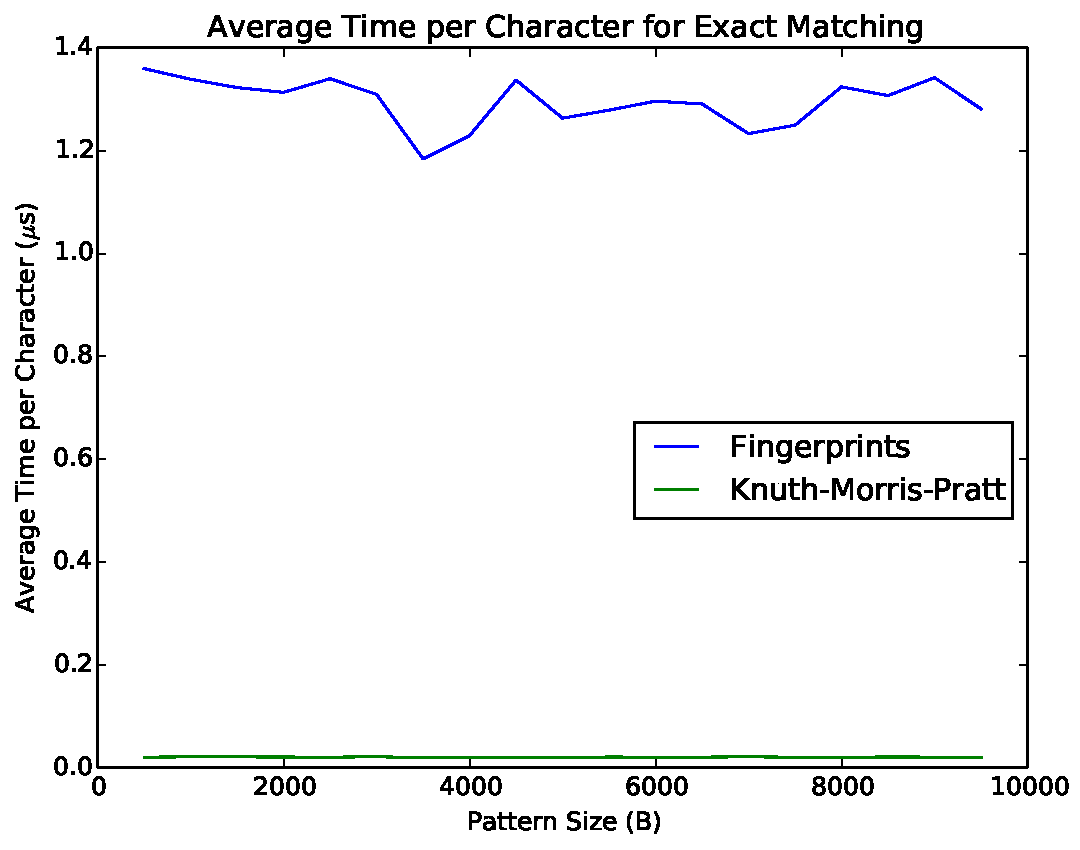
\includegraphics[width=0.5\linewidth]{summer_run_time}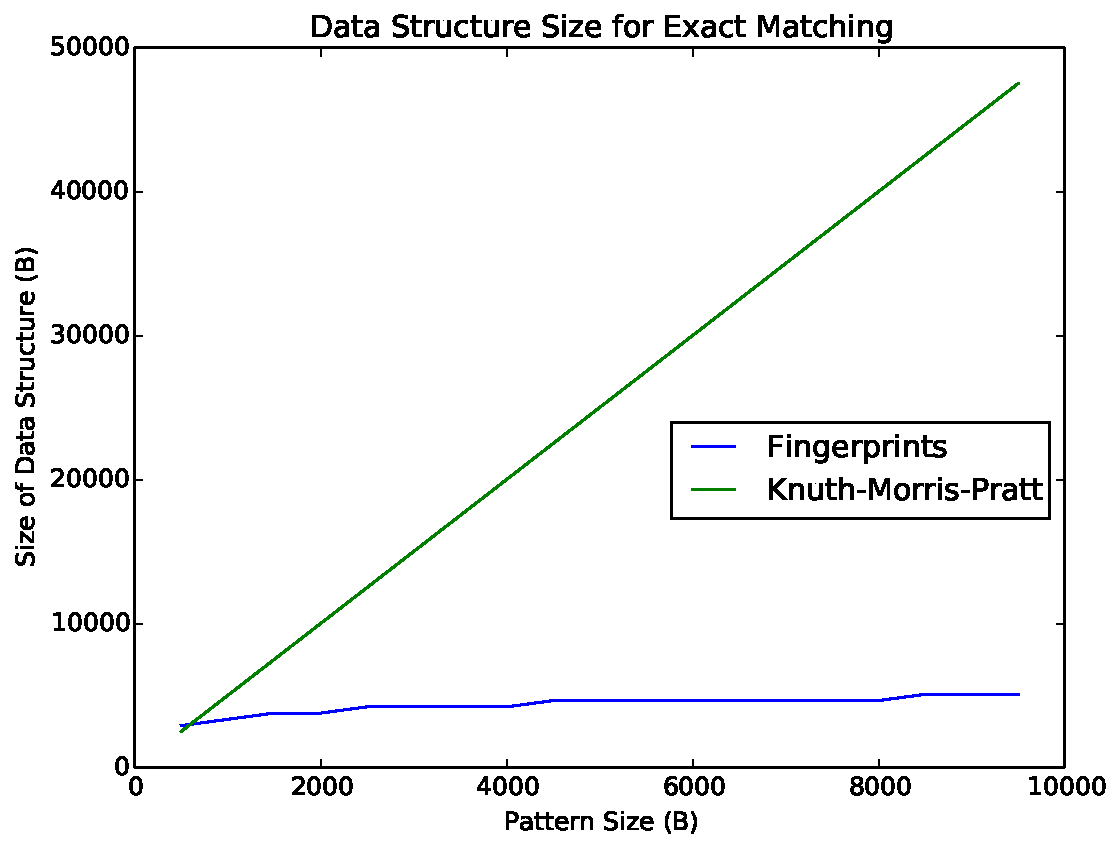
\includegraphics[width=0.5\linewidth]{summer_size}
\end{center}
\caption{Run time and space performance for Breslauer and Galil's algorithm against Knuth-Morris-Pratt}
\label{fig:summer-results}
\end{figure}

\section{Clifford, Fontaine, Porat and Sach: Dictionary Matching in Sublinear Space}
\label{sec:theory-clifford}

Clifford et al.\cite{clifford:dict-matching} provided a solution to dictionary matching under the streaming model in less space than it takes to store the pattern. Their solution uses $O(k\log m)$ space and $O(\log m)$ time per character, where $m = \max(M)$. It is worth noting that this description is based off of a version of this paper that was not accept, and the accepted version of the paper will likely have some differences to what is described here. Also note that these are how the algorithm is described in the paper; any changes to how the algorithm works in later chapters are my own work to correct the algorithm.

The first step to understanding the algorithm as described in the paper is to consider a subset of the dictionary matching problem, where all the patterns are a power of two in length. This algorithm is very similar to the one described in Section~\ref{sec:porat-porat}, where all the patterns are broken up into $\log m_i$ fingerprints, denoted $\phi_{i,j}$ and defined as follows:

$$\phi{i,j} = \phi(p_{i,0}...p_{i,2^j-1})$$

Each level of the algorithm now contains up to $k$ of these prefix fingerprints, and stores all of them in a static perfect hash table. Along with this, each level stores up to $k$ aritmetic progressions of viable occurrences. When the next character enters the stream, each level checks if one of the arithmetic progressions has a viable occurrence that requires processing. If there is, then the algorithm uses static perfect hashing to check if the last $2^j$ characters in the text match any of the prefixes at that level. If there is a match, that VO is promoted to the next level. Finally, a flag is also specified in the hash table to indicate if the given fingerprint is actually the fingerprint of a whole pattern. If that flag is true, then a match at that index is reported.

In terms of complexity, each level requires $O(k)$ space and there are $\log m$ levels, so space usage is $O(k\log m)$ as required. Time complexity depends on how long it takes to figure out if an arithmetic progression needs processing and if so which one. Assuming this can be done in constant time, then each level takes constant time and thus an overall performance of $O(\log m)$ time per character is given.

In order to go from this to the general case of any length of pattern, the patterns are broken up into three cases, based on their length $m_i$ and period $\rho_i = \rho_{P_i}$:

$$|\rho_i| \geq k; (m_i \geq k \text{ and } |\rho_i| < k); m_i < k$$

\subsection{Patterns with Long Periods}

We start with the case where for every pattern $P_i$ in our dictionary $|\rho_i| \geq k$. We start by defining $Q_i$ to be the $m_i - k$ prefix of the $i$-th pattern. For this algorithm to work, we continue under the assumption that $|\rho_{Q_i}| \geq k$. We will see a brief solution for when this assumption does not hold in the subsubsection at the end of this case.

The first part of this case works the same as in the power of two length case. We perform the above algorithm on $\log|Q|$ levels, where $Q$ is the prefix of the longest pattern. If there is a match at a given level, we insert the viable occurrence that matched into a special row, which stores one arithmetic progression for each prefix. At each text index $j$, we process two prefixes. Let $Q_i$ be one of those prefixes processed at $j$, and we perform the following:

\begin{enumerate}
  \item First, if $j \geq l + |Q_i|$, where $l$ is the location of the VO stored in the arithmetic progression related to $Q_i$, then we check if $\phi(t_{l+1}...t_{l+Q_i+1}) = \phi(Q_i)$. In other words, did the $|Q_i|$ characters following the VO location match the prefix?
  \item If there is a match, then we insert all the fingerprints for the $k$ length suffixes of all the patterns in the dictionary for which $Q_i$ is a prefix into a binary search tree (BST). The binary search tree is set up so that it will only be queried when the stream reaches index $l + |Q_i| + k$.
\end{enumerate}

Finally, the algorithm checks to see if any binary search trees need processing. If so, the algorithm takes the fingerprint of the last $k$ characters seen in the stream, and searches the BST to see if a match is found. If a match is found, then an entire pattern has been matched, and the index $j$ is returned.

Time complexity wise, processing the power of two length prefixes costs $O(\log|Q|)$ time per character by simply substituting $m = |Q|$ into the previous definitions. The first step of processing each prefix takes constant time, but may be delayed by up to $\frac{k}{2}$ characters. The second step is more complicated, and in the worst case -- where all the patterns have the same $m_i - k$ length prefix -- will take $O(k\log k)$ time per character if implemented na\"{i}vely. However, because of our assumption that $\forall i, |\rho_{Q_i}| \geq k$, each prefix can only occur once every $k$ characters. This means that, amortised over $k$ characters, our time complexity becomes $O(\log k)$ time per character. Furthermore, this can be deamortised by inserting two suffixes into the BST per index, bringing our worst case time complexity for this step down to $O(\log k)$ per character. Steps 1 and 2 are both delayed by at most $\frac{k}{2}$ indexes each, so the overall delay will be at most $k$ indexes, within time for the BST to be processed. Finally, searching the BST takes $O(\log k)$ time. Putting all of this together gives us $O(\log|Q| + \log k)$ time per character, and because of our assumption that $\rho_Q \geq l$, this becomes $O(\log|Q|) \in O(\log m)$ time per character.

As for space usage, the power of two length prefixes uses $O(k\log|Q|)$ space. Storing the fingerprints of all the prefixes costs $O(k)$ space, as does storing lists of all the suffixes. To cater for both the $\frac{k}{2}$ delay in the first step of the prefix processing and searching for the fingerprint of the last $k$ characters in a BST, we store a circular buffer of the last $k$ fingerprints, which takes up $O(k)$ space. Finally, we may need up to $k$ binary search trees, and at any given time the total number of nodes across all BSTs is at most $k$, so this again is $O(k)$ space. This gives us an overall space usage of $O(k\log|Q|) \in O(k\log m)$ space.

\subsubsection{An Edge Case}
\label{sssec:edge-case-theory}

As previously mentioned, there is an edge case in the above algorithm if $\exists i \text{ such that } |\rho_{Q_i}| < k$. Any patterns which fall under this case can be processed by using the algorithm for long patterns with short periods described in Section~\ref{ssec:periodic-theory} to process their prefix $Q_i$. Any matches returned from this algorithm can be extended from $m_i - k$ to $m_i$ by a combination of fingerprinting and static perfect hashing.

\subsection{Long Patterns with Short Periods}
\label{ssec:periodic-theory}

The next case detailed is where the patterns in the dictionary are longer than $k$, but their periods are shorter. In this algorithm, we store a fingerprint of the $k$ length prefix of each pattern, and call the result $K_i$. For each $K_i$, we store a fingerprint of the period of the pattern $\phi(\rho_i)$ and the period's length $|rho_i|$ along with a counter of the number of times it has occurred the index of the last time it occurred in the current arithmetic progression and the fingerprint of the text at the last occurrence.

When a new index comes in, we use a static perfect hash function to check if the fingerprint of the last $k$ characters in the text stream matches some $K_i$. If so, we check if this index fits in with the rest of $K_i$'s arithmetic progression by checking the current index is $|\rho_i|$ characters away from the last occurrence and the fingerprint suffix of the current stream with the fingerprint of the stream at the last occurrence matches the fingerprint of the period. If they do match then we increment the counter, otherwise we abandon the arithmetic progression by resetting the counter to 1 and setting the last occurrence to the current index and fingerprint.

The second step we perform is to check if the fingerprint of the last $k$ characters in the text matches the last $k$ characters in one of the patterns -- referred to as the \textit{tail} of each pattern. This can be done by storing the fingerprint of the tails of each pattern in another static perfect hash table.

At this point, we are going to assume that no patterns are a suffix of another pattern. If this is not the case, then it is possible to perform dictionary matching, but it comes at the cost of not knowing which patterns have matched. This is why for our choice of dictionary matching, we do not care about what pattern(s) have matched. It is also why we can only return the index at the end of the instance; the only way we could know the starting index of the would be if we knew what the pattern was, since then we could just simply take the current index and subtract the length of the pattern.

Anyway, either through no pattern being a suffix of any other pattern or through discarding the patterns which do have other patterns as suffixes, we end up in a situation where each pattern has a unique tail. If the last $k$ characters in the stream match the tail of some pattern $P_i$, we check the arithmetic progression associated with that pattern. In order for a match to have occured, there need to have been at least $\lfloor\frac{m_i}{\rho_i}\rfloor$ occurrences of $K_i$ in the progression, and the last occurrence must have happened $m_i \mod \rho_i$ characters ago. If both of these conditions hold, then a match is reported.

Complexity wise, the progressions can be stored in $O(k)$ space, as can the fingerprints of the tails. The fingerprint of the last $k$ characters in the text stream can be stored by using a circular array of such fingerprints for the last $k$ indexes. Thus space usage is $O(k)$. As for time, the static perfect hashing operations are constant time, as is inserting the occurrence into the arithmetic progressions and checking for a match, so time overall is $O(1)$.

\subsection{Short Patterns}

The final case to consider is where all the patterns are shorter than $k$. The algorithm for this case is an adaptation of binary search, searching over suffixes of the stream of lengths from 1 to $k$ to see if a pattern matches any of them. However, binary search cannot be applied na\"{i}vely, as we may need to search both parts of the search space. Instead, we use a hash table with a fingerprint as the key and a boolean as the value to find out which half of the space to search.

Algorithm~\ref{alg:short-dict-matching} computes the hash table that is used. We call $\mathtt{PreProc}(k',m_i)$ on each pattern $P_i$, where $k'$ is the nearest integer power of two no smaller than $k$. Note that $\mathcal{S}$ is a boolean function which, given a string, returns True if there is a pattern in the dictionary which is a suffix of that string, and False otherwise.

\begin{algorithm}[t]
\uIf {$y \geq x/2$} {
  $\mathcal{H}_3.\text{insert}(\phi(p_{m_i-x/2}...p_{m_i}), \mathcal{S}(p_{m_i-x/2}...p_{m_i}))$\\
  $\mathtt{PreProc}(x/2,y - x/2)$
}
\Else {
  $\mathtt{PreProc}(x/2,y)$
}
\caption{$\mathtt{PreProc}(x,y)$: Preprocessing of a single pattern}
\label{alg:short-dict-matching}
\end{algorithm}

At each index $j$, we keep a cyclic buffer of the previous $k'$ fingerprints of the whole stream. We start our binary search by seeing if $\phi(t_{j - k/2 + 1}...t_j)$ is within the hash table and its associated boolean value. If the boolean value is True, we know that there is an occurance of the pattern which ends at this index, so we report it. If the boolean value is false but the key exists in the table, then we know that this fingerprint matches the suffix of a pattern, but not necessarily all of it, so we check the longer suffixes of the text. If there is no key in the table, then we know that no pattern matches this suffix, but they might match shorter ones, so we check shorter suffixes instead. This continues until we either report an instance or run out of search space.

For space complexity, the only space used is the hash function which uses $O(k\log k)$ space to store the fingerprints and their associated booleans and the cyclic buffer, which uses $O(k') \in O(2k) \in O(k)$ space, so the overall space usage is $O(k\log k)$. The only step in the algorithm is the binary search, which takes $O(\log k)$ time per character.

% -----------------------------------------------------------------------------

\chapter{Project Execution}
\label{chap:execution}

\section{Implementing the Aho-Corasick Algoritm}

\subsection{From Knuth-Morris-Pratt to Aho-Corasick}

As stated in Section~\ref{sec:aho-corasick}, Aho-Corasick\cite{Aho:1975:ESM:360825.360855} is a generalisation of Knuth-Morris-Pratt. Because of this, I decided the most suitable way of attempting to implement this algorithm was to start with an implementation of KMP and then generalise it to $k$ patterns.

Most implementations of KMP simply consist of an array of $m$ integers to act as a failure table, a string of $m$ characters for the pattern, and a counter of the number of characters that have matched so far, with the counter reaching $m - 1$ representing the accept state. But this is actually a simplification of the algorithm. As pointed out in CLRS\cite{clrs:kmp}, the correctness of Knuth-Morris-Pratt can be proven because this array, string and integer represent a finite state automaton: The array of integers represent the state the automaton should fall back to if the pattern does not match, the string shows the next character that needs to arrive in the text in order for the automaton to move one state closer to the accept state, and the counter represents the current state the automaton is in, with $m - 1$ being the accept state of the automaton.

We can show this with an example: Table~\ref{tab:kmp-pattern-failure} shows the pattern and failure table for the pattern $aabab$, and Figure~\ref{fig:kmp-pattern-failure} shows the state transition diagram for the same pattern.

\begin{table}[t]
  \centering
  \begin{tabular}{|l|c|c|c|c|c|}
    \hline
    \textbf{Index} & 0 & 1 & 2 & 3 & 4 \\\hline
    \textbf{Pattern} & $a$ & $a$ & $b$ & $a$ & $b$ \\\hline
    \textbf{Failure} & -1 & 0 & -1 & 0 & -1\\\hline
  \end{tabular}
  \caption{Pattern and failure table for pattern $aabab$}
  \label{tab:kmp-pattern-failure}
\end{table}

\begin{figure}[t]
  \centering
    \begin{tikzpicture}[node distance=2cm,on grid,auto]
      \node[state] (start) at (0,0) {-1};
      \node[state] (0) [right of=start] {0};
      \node[state] (1) [right of=0] {1};
      \node[state] (2) [right of=1] {2};
      \node[state] (3) [right of=2] {3};
      \node[accepting, state] (4) [right of=3] {4};
      \path[->]
        (start) edge node {$\{a\}$} (0)
        (0) edge node {$\{a\}$} (1)
        (1) edge node {$\{b\}$} (2)
        (2) edge node {$\{a\}$} (3)
        (3) edge node {$\{b\}$} (4)
        (start) edge [loop left] node {$\Sigma/\{a\}$} (start)
        (0) edge [bend left] node {$\Sigma/\{a\}$} (start)
        (1) edge [bend left] node {$\Sigma/\{b\}$} (0)
        (2) edge [bend right] node {$\Sigma/\{a\}$} (start)
        (3) edge [bend left] node {$\Sigma/\{b\}$} (0.south)
        (4) edge [bend left] node {$\Sigma$} (start.south);
    \end{tikzpicture}
  \caption{State transition diagram for pattern $aabab$. Edges directed right represent matches, edges directed left represent failures.}
  \label{fig:kmp-pattern-failure}
\end{figure}

Because the Aho-Corasick algorithm generalises Knuth-Morris-Pratt by taking this finite automaton and adapting it for multiple patterns, I decided a suitable way of starting the project was to implement KMP as a finite automaton.

This meant an important first decision to make: How to implement the automaton? As a finite state automaton is based on graphs, there are three main options available:

\begin{itemize}
  \item \textbf{Adjacency Matrix:} An item at coordinates $(i,a)$ in the matrix represents an edge in the matrix from state $i$ if the next character is $a$. The value of $(i,j)$ itself is the $\texttt{goto}$ state, and is set to the failure state if there is no subsequent pattern with the next character in the state. Constant time travelling between states but $O(m|\Sigma|)$ space.
  \item \textbf{Adjacency List:} Each item in the list is a tuple $(i, j, a)$, representing an edge from $i$ to $j$ if $a$ is next on the tape. Failure edges are represented by an integer for each state. Potentially less space than an adjacency matrix but $O(m * \min(|\Sigma|, m))$ time to move to $\texttt{goto}$ state.
  \item \textbf{Object Oriented:} A state structure is defined, with an array of pointers to other states it connects to and the next character that needs to be read on the tape for the automaton to enter that state. Failure edges are simply a pointer to failure state. Performance is a compromise between an adjacency matrix and an adjacency list, with the same asymptotic space consumption as an adjacency list but $O(\min(|\Sigma|, m))$ time to move to $\texttt{goto}$ state.
\end{itemize}

My initial decision was to use the object oriented approach. Implementing Knuth-Morris-Pratt in this form is easy: When constructing the $\texttt{goto}$ edge, we just iterate through each character in the pattern and connect a new state to the most recent state made. When both constructing the failure pointer and processing the text, we just use the standard KMP algorithm, only using pointers to states instead of integers. And when destroying the automaton at the end, we just recursively call the destroy function on the $\texttt{goto}$ item in the automaton. Note that we don't worry about destroying the node pointed to along the failure edge, as we know that will be destroyed later.

However, while this method was simple enough for KMP, generalising it for Aho-Corasick led to a number of memory problems. In particular, there were issues with the starting state of the automaton being overwritten by another node later on, leading to corrupted memory and double free attempts. The conclusion was that this was too problematic an implementation of automaton for C.

In the end, a hybrid method was used for representing the automaton, combining adjacency matrices with the object oriented approach. The current state is simply represented by an integer, the $\texttt{goto}$ state is represented by a 2-D array of integers $\texttt{goto}$, the character it needs to match is represented by an array of strings $\texttt{match}$ and the failure edges represented by an array of integers $\texttt{failure}$. Thus if we're in state $i$ and character $a$ is the next character in the text, the next state we move to is determined by:

\[
  \begin{cases}
    \texttt{goto}(i, j),& \text{if } \exists j \text{ such that } \texttt{match}_i(j) = a\\
    \texttt{failure}(i),& \text{otherwise}
  \end{cases}
\]

This has the same performance as the object oriented approach, both in terms of time and space.

One detail to remember is that the current state is the index of several arrays. Thus, we cannot have our start state as -1 anymore. This is easy to remedy however, by just having the start state be 0 instead. This is the only discrepancy between our terms for KMP above and our work on Aho-Corasick below.

\subsection{Removing the $\Sigma$ Dependency from Preprocessing}
\label{ssec:ac-hashing}

One of the major problems with the Aho-Corasick algorithm as it is defined in Section~\ref{sec:aho-corasick} is that Algorthms~\ref{alg:ac-goto}, \ref{alg:ac-failure} and \ref{alg:ac-next} all rely on us knowing the complete alphabet at preprocessing time. This is not guaranteed under the streaming model, and requires multiple passes over the text and pattern.

In order to cater for this, a few changes have been made to each algorithm. For Algorithm~\ref{alg:ac-goto}, we change it by specifying the result the output from $\texttt{goto}$ if the next character does not match $failure = 0$. This removes the need for the final loop entirely on that case.

For Algorithm~\ref{alg:ac-failure}, we already know for every state $i$ every character $a \in \Sigma$ such that $\texttt{goto}(i, a) \neq fail$. That is because all of these characters are stored in the $\texttt{match}$ strings, so we can simply iterate through each state's associated string.

Algorithm~\ref{alg:ac-next} is the hardest to remove the alphabet dependency for, but it is still acievable. For the first loop, we only iterate over the characters in state 0's $\texttt{match}_{0}$ string, and set $\texttt{next}(i, a) = 0$ by default. For any other state, denoted $i$, we start by handling the case where $\texttt{goto}(i, a) \neq fail$, by simply iterating through the characters stored in the $\texttt{match}_i$ strings. We then handle the other case by iterating through every character $a \in \texttt{next\_chr}_{\texttt{failure}(i)}$, where $\texttt{next\_chr}_i$ is the string of characters for state $i$'s $\texttt{next}$ function: if $a \notin \texttt{match}_i$, then we know that $\texttt{goto}(i, a) = fail$. If $\exists a \in \Sigma \text{ such that } a \notin \texttt{match}_i \cup \texttt{next\_chr}_{\texttt{failure}(i)}$, it must hold that $\texttt{next}(i, a) = 0$, as it does by default, so we do not need to worry about these characters.

\subsection{Removing the $|\Sigma|$ Run Time per Character}

The bottleneck with Aho-Corasick at processing time is that for our current state, we need to compute the $\texttt{next}$ function. This is not easy to implement; the simplest implementation is linear search, as described in Algorithm~\ref{alg:ac-search}, which would take $O(|\Sigma|)$ time per character. A more efficient implementation could use a binary search tree, which would be $O(\log|\Sigma|)$, but there is in fact an even better way.

\begin{algorithm}[t]
\For{$i=0$ {\bf upto} $|\texttt{next\_chr}_i|$}{
  \If{$\texttt{next\_chr}_i(j) = a$}{
    {\bf return} $\texttt{next\_state}_i(j)$
  }
}
{\bf return} 0
\caption{Computing the $\texttt{next}(i, a)$ function by linear search.}
\label{alg:ac-search}
\end{algorithm}

Note that after preprocessing, we never add any characters to or remove any characters from $\texttt{next\_chr}_i$. As a matter of fact, the $\texttt{next}$ function does not change at all after preprocessing has completed. This means that we can compute this function by having a static perfect hash table for each state $i$, with $\texttt{next\_chr}_i$ as the keys and $\texttt{next\_state}_i$ as the values. This gives uss constant time per character.

For implementation, I used the C Minimum Perfect Hashing Library (CMPH) configured to the Compress, Hash and Digest algorithm (CHD). This was contained in a data structure based on my summer project as mentioned in Section~\ref{sec:summer}. One of these three cases occurs when a structure is searched with key $key$:

\begin{enumerate}
  \item If there are no keys and values for a hash table, return 0 by default.
  \item If there is one key, check if $keys_0 = key$ and if so return $values_0$, if not return 0.
  \item Otherwise, do a CMPH search on the key. If none of the keys match the search key, CMPH will by default return either the number of keys or the index of some key. If it returns the index of some key $i$, check if $keys_i = key$. If they match, return $values_i$, otherwise return 0.
\end{enumerate}

Because the keys are a single character, each search can be evaluated in constant time. Since we are implementing the $\texttt{next}$ function, we only need to call one search per index. Thus the overall run time per character for the algorithm is now constant time. The hash function takes up the same amount of space as the $\texttt{next}$ function would, as does the rest of the search structure, as we are using a minimum perfect hash function. There are only as many search structures are there are states, so we are left with the same space usage as traditional Aho-Corasick.

\subsection{A Brief Note on $\texttt{output}$}

Aho-Corasick offers the advantage that we can return what patterns matched at a given index. However, due to limitations on the Clifford et al. algorithm described in \ref{ssec:periodic-theory}, we only care about \textit{if} a pattern matched, regardless of \textit{which} pattern(s) matched. Because of this, the $\texttt{output}$ function was changed from returning a set to returning an integer, with 0 to represent no patterns matching and 1 to represent a match.

This change requires two lines of the algorithm being modified:

\begin{enumerate}
  \item Line 15 of Algorithm~\ref{alg:ac-goto} becomes $\texttt{output}(state) = 1$
  \item Line 15 of Algorithm~\ref{alg:ac-failure} becomes $\texttt{output}(state) = \texttt{output}(state) \vee \texttt{output}(\texttt{failure}(state))$
\end{enumerate}

If unspecified, $\texttt{output}(state)$ is 0 by default.

\section{Implementing the Clifford et al. Algorithm for Power of Two Length Dictionary Matching}

The rest of this chapter describes the implementation of Clifford, Fontaine, Porat and Sach's algorithm as described in Section~\ref{sec:theory-clifford}. Note that, this algorithm does not achieve $O(\log m)$ time per character as desired, but $O(\log k\log m)$ instead. The reason behind this will be explained later in this section. It is also worth noting, as will be explained in Section~\ref{sec:impl-long} that this is amortised time per character; the real time per character is $O(\log k(k + \log m))$.

\subsection{Implementing Karp and Rabin's Algorithm for Dictionary Matching}

I decided a good start to implementing the algorithm for dictionary matching with fingerprints was to first investigate the algorithm described in Section~\ref{sec:kr-fingerprints} for dictionary matching when all patterns are the same length $m$, based off of Karp and Rabin's original algorithm. This is because it is a simpler algorithm to implement than Clifford et al., yet both require similar libraries: One for static perfect hashing and one for Karp-Rabin fingerprints.

Using these libraries, implemented as described in the two sections below, Karp and Rabin's algorithm was simple to implement. The static percfect hash function contained fingerprints of all the patterns. We stored a fingerprint of the last $m$ characters, and update it by concatenation and suffix operations using a circular buffer of the last $m$ characters. This offers $O(k + m)$ space and $O(1)$ time per character, as mentioned before.

\subsubsection{Implementing Karp-Rabin Fingerprints}

The library for Karp-Rabin fingerprints was written using the GNU Multiple-Precision Arithmetic Library (GMP) version 6.0.0 for the C programming language.

There are two reasons for using GMP:
\begin{enumerate}
  \item It allows for fingerprints and primes to be of any size.
  \item Picking a prime number is fast and doesn't require implementation itself, due to the $\texttt{mpz\_nextprime}$ function.
\end{enumerate}

The cost is that multiple precision operations are typically slower than standard 32/64-bit arithmetic. It was decided that this was a worthwhile drawback however, as we cared about the data tested on being large.

The library itself was based off of my summer project described in Section~\ref{sec:summer}, and consisted of two structures described below.

The first structure, called a fingerprinter, consists of two multiple precision integers $p$ and $r$. When initialised, the fingerprinter takes as input the length of the text $n$, uses GMP to work out $n^2$ and then $\texttt{mpz\_nextprime}(n^2)$ to pick a prime number $p$.

The integer $r$ is where this library most significantly differs from my summer project. For both implementations, entropy is gathered by reading in data from $/dev/urandom$ and then used to seet the GMP. For the summer project, the integer $r$ was picked using the Mersenne Twister function on $\texttt{mpz\_urandomm}$ with maximum being $p$. But this is not guaranteed to work, as it allows two problematic cases:

\begin{itemize}
  \item If $r = 0$, then $\phi(S) = \phi(S')$ if $s_0 = s'_0$.
  \item If $r = 1$, then $\phi(S) = \phi(S')$ if $S$ is a reordering of the characters in $S'$.
\end{itemize}

To avoid these two cases, $\texttt{mpz\_urandomm}$ is still used, but the maximum is now set as $p-2$. This will generate a number $r$ such that $0 \leq r < p-2$. Incrementing $r$ by 2 gives us $2 \leq r < p$. This means that the fingerprints will not work if $p = 2$, but this is only the case if $n = 1$, in which case the text is one character long and can just be matched na\"{i}vely.

The second structure, called a fingerprint, consists of three multiple precision integers: $\texttt{finger}$ refers to the fingerprint of the string itself $\phi(S)$ for a $k$ character string $S$, $\texttt{r\_k}$, which refers to $r^k$, and $\texttt{r\_mk}$, which refers to $r^{-k}$.

After space has been allocated, the fingerprints of strings can be computed by a function called $\texttt{set\_fingerprint}$. This function is implemented as the equation in Section~\ref{sec:kr-fingerprints}, and based off of the work from my summer project. However, again there was a problem with my summer project's implementation, where the first item was not being computed modulo $p$. This meant that, if the string $S$ was 1 character long and $s_0 \geq p$--a case which is easily possible depending on the encoding of the characters in the string and if $p$ is sufficiently small--then $\phi(S) \geq p$. This was easily fixed by simply adding an additional modulo statement for the first character of the string. $r^k$ was calculated incrementally as $r*r*r*...*r$, as we required $r^0,r^1...,r^{k-1}$ for computing the fingerprint, and $r^{-k}$ was calculated using $\texttt{mpz\_invert}$ on $r^k$.

Concatenation, prefix and suffix operations are computed as shown in Section~\ref{sec:kr-fingerprints}. The only difference is that, as with setting the fingerprint, $r^{-k}$ was calculated using $\texttt{mpz\_invert}$.

\subsubsection{Implementing Static Perfect Hashing of Fingerprints}

The data structure is similar to the static hash table used for Aho-Corasick, only with fingerprints instead of characters for the keys, and returning the index calculated by the hash function (or $-1$ by default) instead of some value. But there is a problem with this method: The C version of CMPH is designed to only take strings as the keys, whereas we want it to run on (multiple precision) integers.

The method taken for solving this problem was to convert the fingerprints into strings, using the function $\texttt{gmp\_snprintf}$. While this had some impact on performance, it was a quick solution in order to make static hashing work on integers. The conclusion was that if it turns out to be a bottleneck at the testing stage, faster implementations of static hashing could be investigated then or suggested as future work depending on the amount of time left.

The fingerprints were converted into strings of their hexadecimal representation to make calculating the maximum size of the string simple. $\texttt{gmp\_snprintf}$ was used specifically to avoid any chances of a buffer overflow, as we specify the maximum number of characters to write to the string. The maximum length of the string was figured out based on the hexadecimal representation of the modulus $p$, since all fingerprints were integers between 0 and $p - 1$ inclusively.

We cannot figure out the number of characters needed to represent $p$ in hexadecimal exactly without testing individual bytes of $p$, but we can approximate it very easily. Because $p$ is a positive multiple-precision integer from GMP, the number of limbs that are used to represent $p$ are specified by the integer $\texttt{\_mp\_size}$. We can multiply this value by $\texttt{sizeof}(\texttt{mp\_limb\_t})$ to get an upper bound on the number of bytes required to represent $p$. Finally, note that a byte can be represented by two hexadecimal digets, so we double this size, and allocate an extra character at the end for the string terminator $\texttt{`\textbackslash0'}$.

Asymptotically, the space is not affected by this change. We only need to store one string in the structure for the key we want to search at a given point--we store this string in order to avoid constantly allocating and freeing space--and this string will take up as much space as $p$, within a constant factor.

\subsection{From Karp-Rabin to Power of Two Length Dictionary Matching}

\subsubsection{Dictionary Matching Where All Patterns are the Same Power of Two Length}

The next step of implementation was to look at patterns which are all the same power of two length. This essentially works as a combination of Porat and Porat's algorithm with the Karp-Rabin algorithm implemented in the previous section.

The first step is to determine the length of the longest pattern $m$, and then use this to compute $\log m$, so that we can allocate enough rows for the pattern. This is done very simply: Iterate through all of the pattern lengths to find the largest, and simply use bit shifting, as shown in Listing~\ref{lst:bit-shift} to compute $\log m$.

\begin{lstlisting}[float={t},caption={Computing $\log m$ via bit shifting.},label={lst:bit-shift},language=C]
while((1 << (matcher->num_rows + 1)) < m_max) {
  matcher->num_rows++;
}
\end{lstlisting}

An interesting question to ask at this point is why we have the +1 in the above listing. This is because the very fist row, which matches prefixes one character long, doesn't need any arithmetic progressions stored. Instead, it just processes those characters live as they come in on the stream.

Because of this, we handle the first row differently. Instead of having an array of progressions for it, we just have a static hash table to check each character $t_j$ as it enters the stream if it matches the prefix of some pattern, and then insert it into level 0 if there is a match. We also don't use the fingerprint static hash table described above for these prefixes. Instead, because these prefixes are only one character long, we use the static hash table used in Section~\ref{ssec:ac-hashing}, which is faster than hashing $\phi(t_j)$.

The rest of the structure is built by iterating through each row $i$ until $2^{i+1} \leq m$, which occurs when $i = \lfloor\log_2m\rfloor$. For row $i$, we iterate through each pattern $P_j$ and create the fingerprint $\phi_{i,j} = \phi(p_{j,0}...p_{j,2^{i + 1} - 1})$. As with Porat and Porat in Section~\ref{sec:porat-porat}, this fingerprint can be created reading each character only once by concatenating the previous prefix with $\phi(p_{j,2^{i}}...p_{j,2^{i + 1} - 1})$.

One point to be cautious of is if different patterns have the same prefix. This can cause problems with CMPH, which does not handle matching keys well, and can also cause later problems for us when looking at different length patterns, if one entire pattern is the prefix for another pattern. We will see this problem arise regularly throughout this project, as all three cases described later in this chapter have the risk of matching fingerprints. In all cases where this issue arises during preprocessing, avoiding this is implemented na\"{i}vely through linear search. A better option would have been to implement it via a binary search tree, but this was only realised after testing was completed.

For each row $i$, we keep count of the number of unique prefixes in that row. We need this information so that when we start building row $i+1$, we know how many arithmetic progressions need to be allocated. For this implementation, it does not matter which prefix in row $i$ is maps via CMPH to which progression in row $i+1$.

This is most of the preprocessing issues explained. The rest of the algorithm works similarly to the way it is described in Section~\ref{sec:theory-clifford}: As each character of the text enters, each row checks if the oldest occurrence stored in any progression can now be tested. If it is tested and succeeds, then it is promoted to the next row and stored using the prefix's period. A few differences are explained below.

Simplest difference first, we do not promote at the final level. Instead, since the final level performs matches against the complete patterns, this level performs a static lookup to see if a full match has occured and if so simply report that match.

The second and more complicated difference is what to do if there is a collision in the fingerprints and thus have a viable occurrence that does not fit with the period. We could use the method suggested by Breslauer and Galil in Section~\ref{sec:porat-porat} and simply report a match every time this happens, but this will cause problems once the patterns are of different lengths since we will not know which index to declare a match at. Instead, this implementation simply ignores such occurrences, and prints a warning on $\texttt{stderr}$ explaining that there was a non-periodic occurrence at this index, which prefix causes the occurrence, and that it has been ignored.

The final difference is how we figure out which arithmetic progression contains the oldest viable occurrence. This detail was omitted from the version of the paper that I was using for this project, and a method for solving this was not devised until it was too late to attempt to implement it. In the original implementation, a simple linear search was performed over the progressions. But this is too costly, as it makes the run time per character to $O(k\log m)$. With that asymptotic performance we might as well just run $k$ copies of the Breslauer and Galil algorithm described in Section~\ref{ssec:breslauer-galil}.

Instead, the next progression was found by using a Red-Black Tree, using source code from \url{http://en.literateprograms.
org/Red-black_tree_(C)?oldid=19567} as a starting point. More precisely, I used a version from my summer project which modified the RBT source code so that when searching the tree, a default value could be specified if the key could not be found. This is because the original implementation of the RBT returns $\texttt{NULL}$ by default, which is problematic as $\texttt{NULL}$ is interpreted by C as 0, and I want to store the value 0 in the tree.

Each row has an RBT as part of its data structure, which takes integers as both keys and values. For key-value pair $i, j$ in a tree, $i$ is the index of the oldest prefix in the $j$-th progression that is yet to be tested. When a viable occurrence is added to an arithmetic progression, a key-value pair is added to the RBT only if that progression was previously empty. Then, when we reach index $i$ in the text, we check the RBT if one of the keys in the tree matches $i$. If so, then progression $j$ can be tested. After testing, we remove $i$ from the RBT, and if the progression $j$ still contains some viable occurrences, insert $(i + |\rho_j|, j)$ into the tree, where $|\rho_j|$ is the length of the period of the $j$-th progression.

There are a few final points worth noting about these trees. First, because the prefixes are the same length, it is impossible to have more than one progression to test for a given index. Thus we have no risk of progressions being lost because of other progressions overwriting them in the RBT. Second, because we only insert items into the tree if either the progression was previously empty or because we have shifted the progression along--which involves deleting an item from the RBT--we have at most $k$ items in the tree at any one time. Thus, we still meet the $k\log m$ space bounds as before.

As for time complexity, inserting, searching and deleting items from the red-black tree take $O(\log k)$ time, where $k$ is the number of items in the tree. We call these functions a constant number of times for each level at each index of the text. Because there are $\log m$ levels to iterate over at each index of the text, the overall runtime is $O(\log k\log m)$, as mentioned at the start of this section.

\subsubsection{Dictionary Matching with Different Power of Two Length Patterns}

From the above implementation, modifying it to handle patterns of different power of two lengths is trivial. For each level, we keep track of an array of integers to indicate if a pattern ends at a given prefix. When preprocessing on pattern $P_j$ at level $i$, we check if $2^{i + 1} = m_j$. If that is the case, then we specify a pattern ending in the array by the value $1$. Otherwise, we use $0$ to indicate that the pattern does not end here. To cater for the case where one pattern is the prefix of another and thus have matching fingerprints, we simply use a bitwise OR to make sure that the array knows that a pattern ends at this prefix.

Finally, the static perfect hash table\footnote{Note that this refers to both the hash tables for fingerprints and the hash table for characters in the first level.} is modified to store these integers, and optionally return them by reference.

Now for each character in the text, we iterate over each level and use the static hash table to check if there is a match with some prefix. Alongside this, we are returned by reference an integer to indicate if a complete pattern matches here or not. If the integer is 1, we report a match at this index, otherwise we report no match.

\section{Implementing the Clifford et al. Algorithm for Short Patterns Dictionary Matching}

\section{Implementing the Clifford et al. Algorithm for Long Patterns with Short Periods Dictionary Matching}

\section{Implementing the Clifford et al. Algorithm for Patterns with Long Periods Dictionary Matching}
\label{sec:impl-long}

% -----------------------------------------------------------------------------

\chapter{Critical Evaluation}
\label{chap:evaluation}

{\bf A topic-specific chapter, of roughly $10$ pages} 
\vspace{1cm} 

\noindent
This chapter is intended to evaluate what you did.  The content is highly 
topic-specific, but for many projects will have flavours of the following:

\begin{enumerate}
\item functional  testing, including analysis and explanation of failure 
      cases,
\item behavioural testing, often including analysis of any results that 
      draw some form of conclusion wrt. the aims and objectives,
      and
\item evaluation of options and decisions within the project, and/or a
      comparison with alternatives.
\end{enumerate}

\noindent
This chapter often acts to differentiate project quality: even if the work
completed is of a high technical quality, critical yet objective evaluation 
and comparison of the outcomes is crucial.  In essence, the reader wants to
learn something, so the worst examples amount to simple statements of fact 
(e.g., ``graph X shows the result is Y''); the best examples are analytical 
and exploratory (e.g., ``graph X shows the result is Y, which means Z; this 
contradicts [1], which may be because I use a different assumption'').  As 
such, both positive {\em and} negative outcomes are valid {\em if} presented 
in a suitable manner.

% -----------------------------------------------------------------------------

\chapter{Conclusion}
\label{chap:conclusion}

{\bf A compulsory chapter, of roughly $2$ pages} 
\vspace{1cm} 

\noindent
The concluding chapter of a dissertation is often underutilised because it 
is too often left too close to the deadline: it is important to allocation
enough attention.  Ideally, the chapter will consist of three parts:

\begin{enumerate}
\item (Re)summarise the main contributions and achievements, in essence
      summing up the content.
\item Clearly state the current project status (e.g., ``X is working, Y 
      is not'') and evaluate what has been achieved with respect to the 
      initial aims and objectives (e.g., ``I completed aim X outlined 
      previously, the evidence for this is within Chapter Y'').  There 
      is no problem including aims which were not completed, but it is 
      important to evaluate and/or justify why this is the case.
\item Outline any open problems or future plans.  Rather than treat this
      only as an exercise in what you {\em could} have done given more 
      time, try to focus on any unexplored options or interesting outcomes
      (e.g., ``my experiment for X gave counter-intuitive results, this 
      could be because Y and would form an interesting area for further 
      study'' or ``users found feature Z of my software difficult to use,
      which is obvious in hindsight but not during at design stage; to 
      resolve this, I could clearly apply the technique of Smith [7]'').
\end{enumerate}

% =============================================================================

% Finally, after the main matter, the back matter is specified.  This is
% typically populated with just the bibliography.  LaTeX deals with these
% in one of two ways, namely
%
% - inline, which roughly means the author specifies entries using the 
%   \bibitem macro and typesets them manually, or
% - using BiBTeX, which means entries are contained in a separate file
%   (which is essentially a databased) then inported; this is the 
%   approach used below, with the databased being dissertation.bib.
%
% Either way, the each entry has a key (or identifier) which can be used
% in the main matter to cite it, e.g., \cite{X}, \cite[Chapter 2}{Y}.

\backmatter

\bibliography{dissertation}

% -----------------------------------------------------------------------------

% The dissertation concludes with a set of (optional) appendicies; these are 
% the same as chapters in a sense, but once signaled as being appendicies via
% the associated macro, LaTeX manages them appropriatly.

\appendix

\chapter{An Example Appendix}
\label{appx:example}

Content which is not central to, but may enhance the dissertation can
be included in one or more appendices; examples include, but are not 
limited to

\begin{itemize}
\item lengthy mathematical proofs, numerical or graphical results
      which are summarised in the main body,
\item sample or example calculations, 
      and
\item results of user studies or questionnaires.
\end{itemize}

\noindent
Note that in line with most research conferences, the marking panel 
is not obliged to read such appendices.

% =============================================================================

\end{document}
